\documentclass[a4paper,12pt]{article}
\usepackage{xeCJK}
\usepackage{listings}
\usepackage{color}
\usepackage{titlesec}
\usepackage{indentfirst}

% meta
\title{汇编语言实验报告}
\author{何柏超}

% fonts
\setCJKmainfont{AR PL New Sung}
\setCJKsansfont{AR PL New Sung}
\setCJKmonofont{WenQuanYi Micro Hei Mono}
\setCJKfamilyfont{hei}{WenQuanYi Micro Hei}

% 隐藏页码
\pagenumbering{gobble}

% 代码样式
\definecolor{comment-green}{rgb}{0,0.6,0}
\lstset {
    basicstyle=\footnotesize\ttfamily,
    language={[x86masm]Assembler},
    tabsize=2,
    numbers=left,
    commentstyle=\itshape\color{comment-green},
}

% 章节样式
\titleformat
{\section}
[block]
{\normalfont\large\bfseries}
{实验 \thesection}
{0ex}
{
    \centering
}
[]
\setcounter{section}{0}

\newcommand{\labtitle}[1] {
    \centerline{
\includegraphics[scale=0.5]{resource/chapter-caption}}

    \begin{tabular}{ l l l }
        \\  % FIXME
        \underline{\hspace{3pt} 计算机学院 \hspace{3pt}} &
            \underline{计算机科学与技术} 专业 \underline{2} 班 &
            学号 \underline{3112005816} \\[3pt]

        姓名 \underline{\hspace{3pt} 何柏超 \hspace{3pt}} &
            协作者 \underline{\hspace{50pt}} &
            教师评定 \underline{\hspace{35pt}} \\[3pt]
    \end{tabular}

    \begin{tabular}{l}
    实验题目\ \underline{#1} \\[3pt]
    \end{tabular}
    \section{#1}
}


\begin{document}

\newcommand{\namefont} {
    \fontsize{16bp}{\baselineskip}\selectfont\CJKfamily{hei}
}

\begin{titlepage}
    \begin{flushleft}
        \hspace{8.5mm}
\includegraphics[height=2.19cm,width=2.21cm]{resource/logo}
    \end{flushleft}
    \begin{center}
        
\includegraphics[height=2.96cm,width=10.56cm]{resource/school}
    \end{center}
    \vspace{6.5mm}
    \begin{center}
        {\fontsize{26bp}{\baselineskip}\selectfont\CJKfamily{hei}{汇编语言实验报告}}
    \end{center}
    \vspace{10mm}
    \begin{center}
        \begin{tabular}{l}
            \fontsize{15bp}{\baselineskip}\selectfont\CJKfamily{hei}{1、 用表格形式显示字符} \\
            \fontsize{15bp}{\baselineskip}\selectfont\CJKfamily{hei}{2、 字母大小写转换} \\
            \fontsize{15bp}{\baselineskip}\selectfont\CJKfamily{hei}{3、 课程设计 \ 1(争优)} \\
        \end{tabular}
    \end{center}
    \vspace{28mm}
    \begin{center}
        \begin{tabular}{r l}
            \namefont{学\hspace{2em}院\hspace{3mm}} & \namefont{\hskip1pt\underline{计算机学院 \hspace{43pt}}} \\[2.5mm]
            \namefont{专\hspace{2em}业\hspace{3mm}} & \namefont{\underline{计算机科学与技术}} \\[2.5mm]
            \namefont{学\hspace{2em}号\hspace{3mm}} & \namefont{\underline{3112005816 \hspace{50pt}}} \\[2.5mm]
            \namefont{学生姓名\hspace{3mm}} & \namefont{\underline{何柏超\hspace{80pt}}} \\[2.5mm]
            \namefont{指导教师\hspace{3mm}} & \namefont{\underline{张\hspace{1em}梅\hspace{80pt}}} \\[2.5mm]
        \end{tabular}
    \end{center}
    \vfill
    \begin{center}
        \namefont{2014 年 11 月 06 日}
    \end{center}
\end{titlepage}


\labtitle{用表格形式显示 ASCII 字符}

\subsection{实验目的与要求}

学习用汇编语言设计与编写循环程序。

\subsection{实验内容}

按 15 行乘 16 列的表格形式显示 ASCII 码为 $10h - 100h$ 的所有字符,
即以行为主的顺序及 ASCII 码递增的次序依次显示对应的字符。
每 16 个字符为一行,每行中的相邻两格字符之间用空格隔开。

\subsection{实验提示}

显示每个字符可使用功能号为 $02h$ 的中断调用,使用方法如下:

\begin{lstlisting}
mov ah, 02h
mov dl, bl ;输出字符的 ASCII 码
int 21h
\end{lstlisting}

本题可把 $dl$ 初始化为 $10h$, 然后不断使其加 1(用 $inc$ 指令)以取得下一个字符的 ASCII 码。
显示空白符时,用其 ASCII 码 $0$ 置入$dl$ 寄存器。每行结束时,\\
用显示回车(ASCII为 $0dh$)和换行符(ASCII为$0ah$)来结束本行并开始下一行。

由于逐个显示相继的ASCII字符时,需要保存并不断修改$dl$寄存器的内容,
而显示空白、回车、换行符时也需要使用$dl$寄存器,为此可使用堆栈来保存相继的ASCII字符。 
具体用法是:
在显示空白或回车、换行符前用指令 \lstinline|push dx| 把 $dl$ 的内容保存到堆栈中去。
在显示空白或回车、换行符后用指令 \lstinline|pop dx| 恢复$dl$寄存器的原始内容。

\pagebreak

\subsection{程序运行截图}

\begin{figure}[h!]
    \caption{实验 1 运行截图}
    \centering
        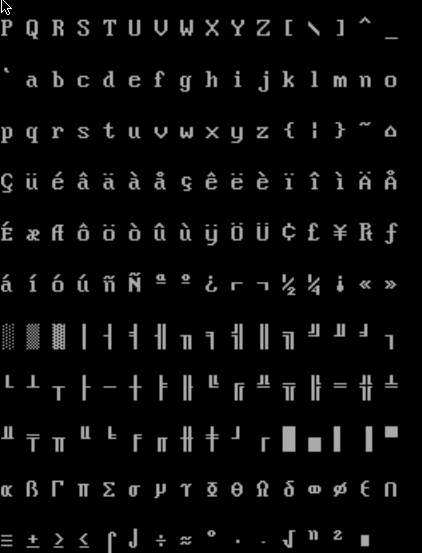
\includegraphics[scale=0.5]{src/2}
\end{figure}

\subsection{程序代码}

\lstinputlisting{src/2.asm}

\clearpage

% ----------------------------------------------------------------------------

\labtitle{字母大小写改写程序}

\subsection{实验要求}

按书中要求编写程序,并将结果显示到屏幕上。

\subsection{程序截图}

\begin{figure}[h!]
    \caption{实验 2 运行截图}
    \centering
        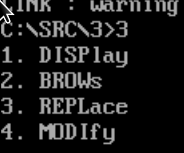
\includegraphics[scale=1]{src/3}
\end{figure}

\subsection{程序代码}

\lstinputlisting{src/3.asm}

\clearpage

% ----------------------------------------------------------------------------

\labtitle{课程设计一}

\subsection{实验要求}

见书上 P211 页。

\subsection{程序代码}

\lstinputlisting{src/4.asm}

\subsection{程序截图}

\begin{figure}[h!]
    \caption{实验 3 运行截图}
    \centering
        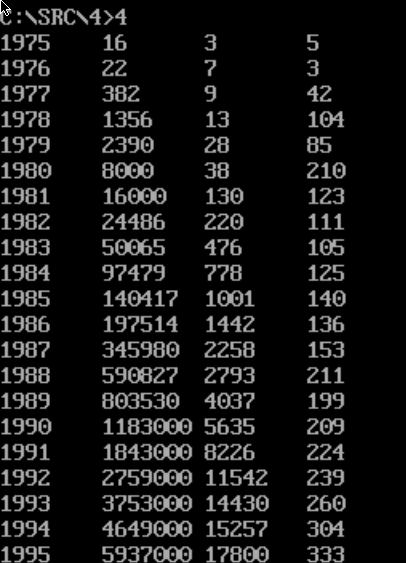
\includegraphics[scale=1]{src/4}
\end{figure}


\clearpage

\end{document}
